\documentclass{article}
\usepackage{graphicx} % Required for inserting images
\usepackage{hyperref}

\title{CSC111: Project 2 report}
\author{Kimberly Prijadi & Jane Felicia Jonatan}
\date{March 2025}

\begin{document}

\maketitle

\section{Project outline}
\begin{itemize}
    \item Project name: \textbf{Laptop Match}
    \item Team members:
    \begin{itemize}
        \item Jane Felicia Jonatan
        \item Kimberly Prijadi
    \end{itemize}
    \item Project goal: \textbf{How can we implement a graph to recommend laptops based on user inputs of price, brand, and laptop specifications?}
\end{itemize}


\section{Project description}
\par Laptops are an indispensable part of our lives, seeing use in various areas including education, business, entertainment, and creative work (CountBarracuda4447, 2024). Most of us in the business world require laptops for mobility in day to day tasks, accessing important information, or communicating with others (Yasir, 2024). It is also very important for those who work or study tech to be able to work on big data and run various computations in a portable manner, thus laptops are now an integral part of our daily lives in this technological society. 
\\
\par However, with the current market, there are many laptop options available for purchase, and we never know if we have found the optimal laptop for our needs. It also proves to be a hassle to look through individual products online just to identify its specifications and compare it with an array of laptops one-by-one. Many people may not even understand tech jargon and be confused with all the specifications that come with laptops. In fact, when 2,392 men and women 18 years of age or older responded to a survey, 11\% of them thought that HTML was an STD, and 23\% thought that MP3 was a Star Wars Robot (Rodriguez, 2014).
\\
\par
As such, \textbf{our goal is to create a useful software for people, both those familiar with tech jargon and not, to get laptop recommendations and find a model replicating what they need, considering their budget, the laptop brand they want, specifications (CPU, RAM, SSD / HDD storage), and display (screen size).}
\\
\par 
The software is user-friendly and straightforward, showcasing an optimal model that meets the user’s needs, along with other similar laptops for the user's consideration. 

\section{Data source}

We used data sourced from: \texttt{Kaggle.com} (Raju, 2023)
\begin{itemize}
    \item Data format: \texttt{.csv}
    \item Source: \href{https://www.kaggle.com/datasets/rajugc/laptop-selection-dataset?resource=download}{Click here!}  % add link perhaps
\end{itemize}

\section{Computational outline}
% Describe the kinds of data your project uses to represent your chosen domain, and how trees and/or graphs play a central role in this data representation.
% Describe the major the computations your program performs, such as: building trees/graphs from a dataset or computation, data transformation/filtering/aggregation, computational models, and/or algorithms.
% Explain how your program reports the results of your computation in a visual and/or interactive way.
% Explain how your program uses Python libraries to accomplish its tasks. Refer to specific functions, data types, and/or capabilities of the library that make it relevant for accomplishing these tasks.

In this project, we used an unweighted graph to represent different laptop and specs nodes then use the graph to calculate the similarity score between our "dummy laptop"/the combination of specs the user wants and other laptops in the graph. When getting data from input boxes, we take note of the kind of data (or specs) (e.g. processor) represented by each empty input box as a list as an additional parameter to calculating the similarity score. Thus, while getting similarity scores of the dummy laptop and all other laptops, when getting the neighbors of other laptops we do not consider vertices representing the "missing specs". The number of factors (or specs) considered is 7 - the length of the list of "missing specs" with 7 being the total number of factors originally considered (minimum and maximum price is counted as 1 factor).
\\
\par
Before we created the graph, we created a data frame using \texttt{pandas} and filtered the data to remove any rows with empty columns as well as any duplicate rows. Some edits were also made to remove laptops with more obscure data for better generality. Furthermore, we converted the price column from INR to CAD with the current exchange rate (0.016) to make it more general for Canadians. We then removed the laptop indexing and reset the count from 0 to ensure ease in creating the algorithm.
\\
\par
Using the finalized data frame, we loaded the graph by creating vertices consisting of ID, laptop name, laptop specs (separated by each category, e.g. processor, processing speed, RAM, etc), laptop price, and reviews. Since the data frame included both processor brand and the type under processor and we want to allow the users to decide processing speed for themselves, we elected to split the data within that column to brand and processing speed using the \texttt{\_convert\_split} function. We then create edges connecting the laptop ID vertex to other vertices. The final graph will show that each laptop ID vertex will be neighbors with their specs vertices.
\\
\par
The program will open up a form allowing users to input their desired specs. There is also a randomize button in case the user does not know what to select. We have also added partial matching in case the user did not fill all parameters, although they will always have to input the limit of how many laptops to generate. Errors are also raised when min price is greater than max price in the user's input, or if they are not floats/integers. Upon the user clicking the Submit button, a 'dummy laptop' with these specs will be created. The dummy laptop vertex is created in a similar fashion as previous laptops and injected into the graph. Then the \texttt{recommend\_laptop} function is run to get similarity scores between the dummy laptop and every other laptop. The results displayed will be the top laptops (1-20; up to user) with the highest similarity score and rating. The most similar laptop will have its specs shown while other laptops will have its name and image shown in grid form. There is also a Back to Form button in case the user wants to return to the main form page and re-enter their desired specs to generate a new set of laptops. Besides that, a quit button is present on the form page to exit the program.
\\
\par
Overall, this program utilises the following python libraries:
\begin{itemize}
    \item \texttt{pandas}: utilizesfilter and transform the csv file data to something usable
    \item \texttt{json}: we used a \texttt{json} file to store unique categories used to categorise the processor and processing speed, RAM, OS, and storage.
    \item \texttt{pygame}: we used that to create the input form as well as the output window.
    \item \texttt{random}: we used this module to generate a \texttt{randint} (random integer) for the randomize button.
    \item \texttt{requests}: we used this module to request images from image urls.
    \item \texttt{typing}: we used Any from this module during function and dataclass attribute creation.
    \item \texttt{io}: we used this module to create a file object for images.
    \item \texttt{python\_ta}: we used this module to check the code for any errors.
    \item \texttt{doctest}: we used this module to check whether the docstring examples run properly.
    \item \texttt{math}: we used math to round up the coordinates for organizing the recommended laptop boxes.
\end{itemize}

\section{Running instructions}
Download the graph\_class.py, laptops.csv, main.py, parameters\_data.json, and user\_input\_form.py.
Install all Python libraries listed under the requirements.txt file.
Then, run the \texttt{main.py} in console.

\section{Expected output}
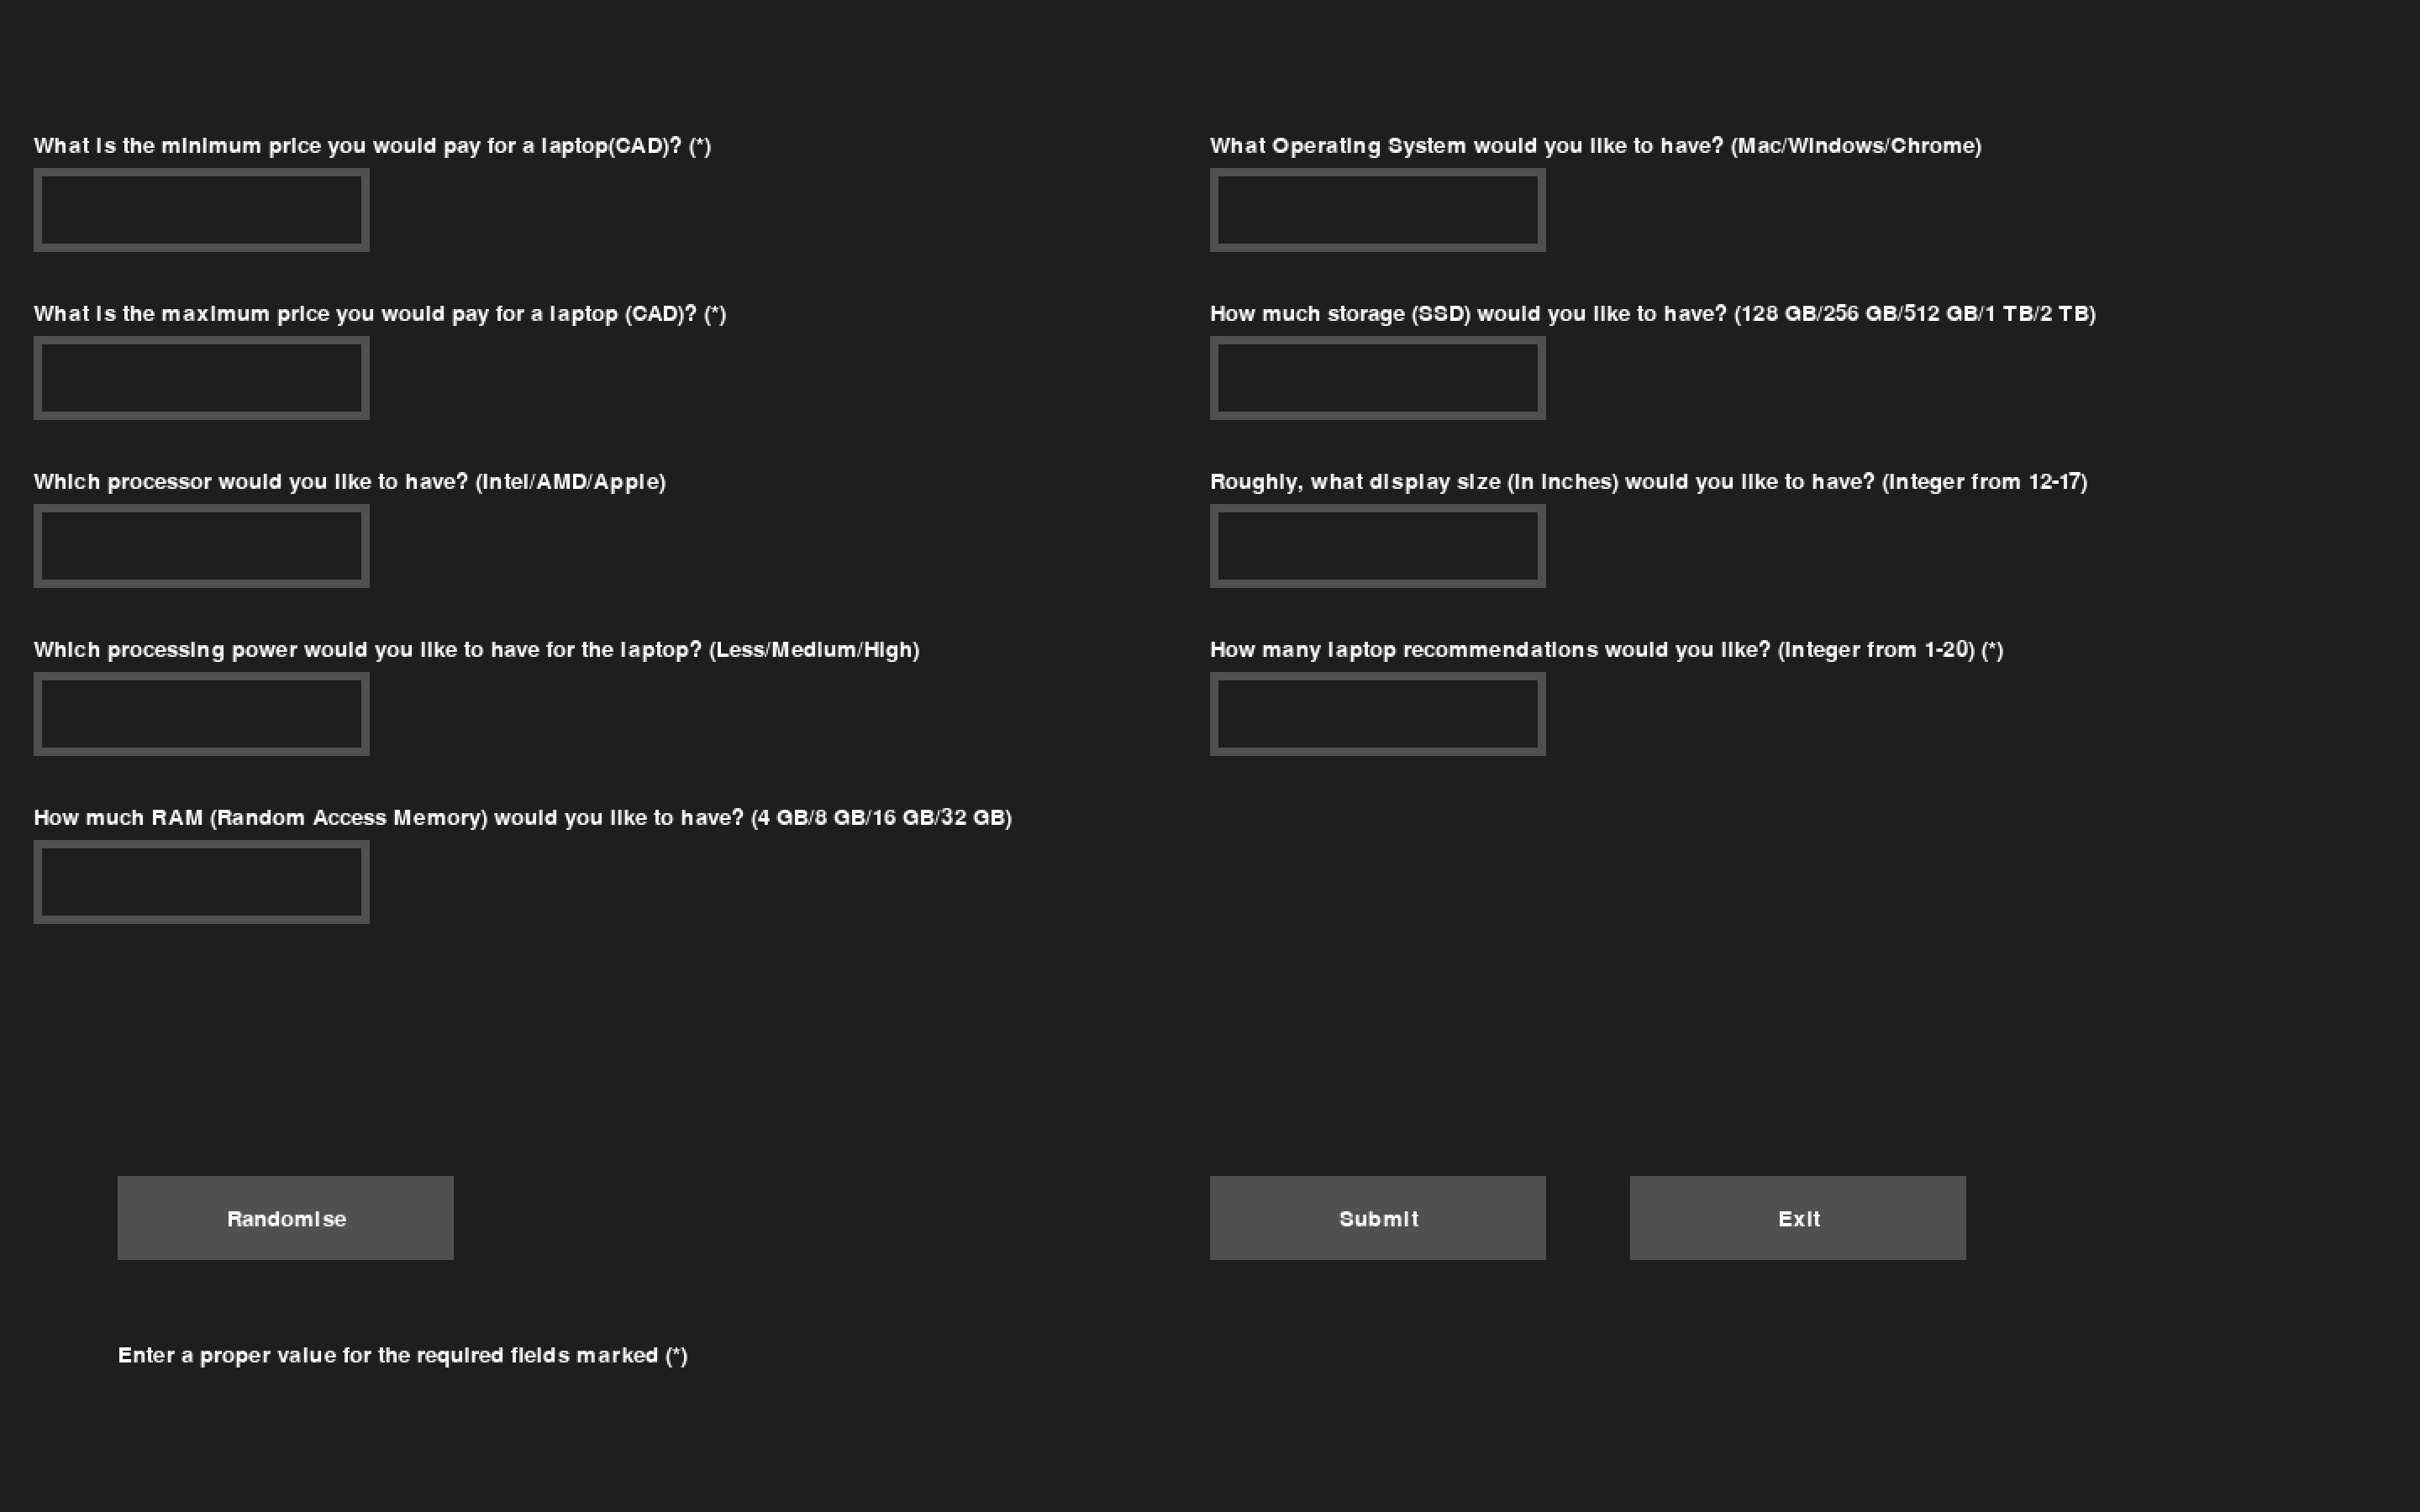
\includegraphics[scale=0.1]{proj2_input_form.png}
\\
\texttt{This is the expected form screen.}
\\
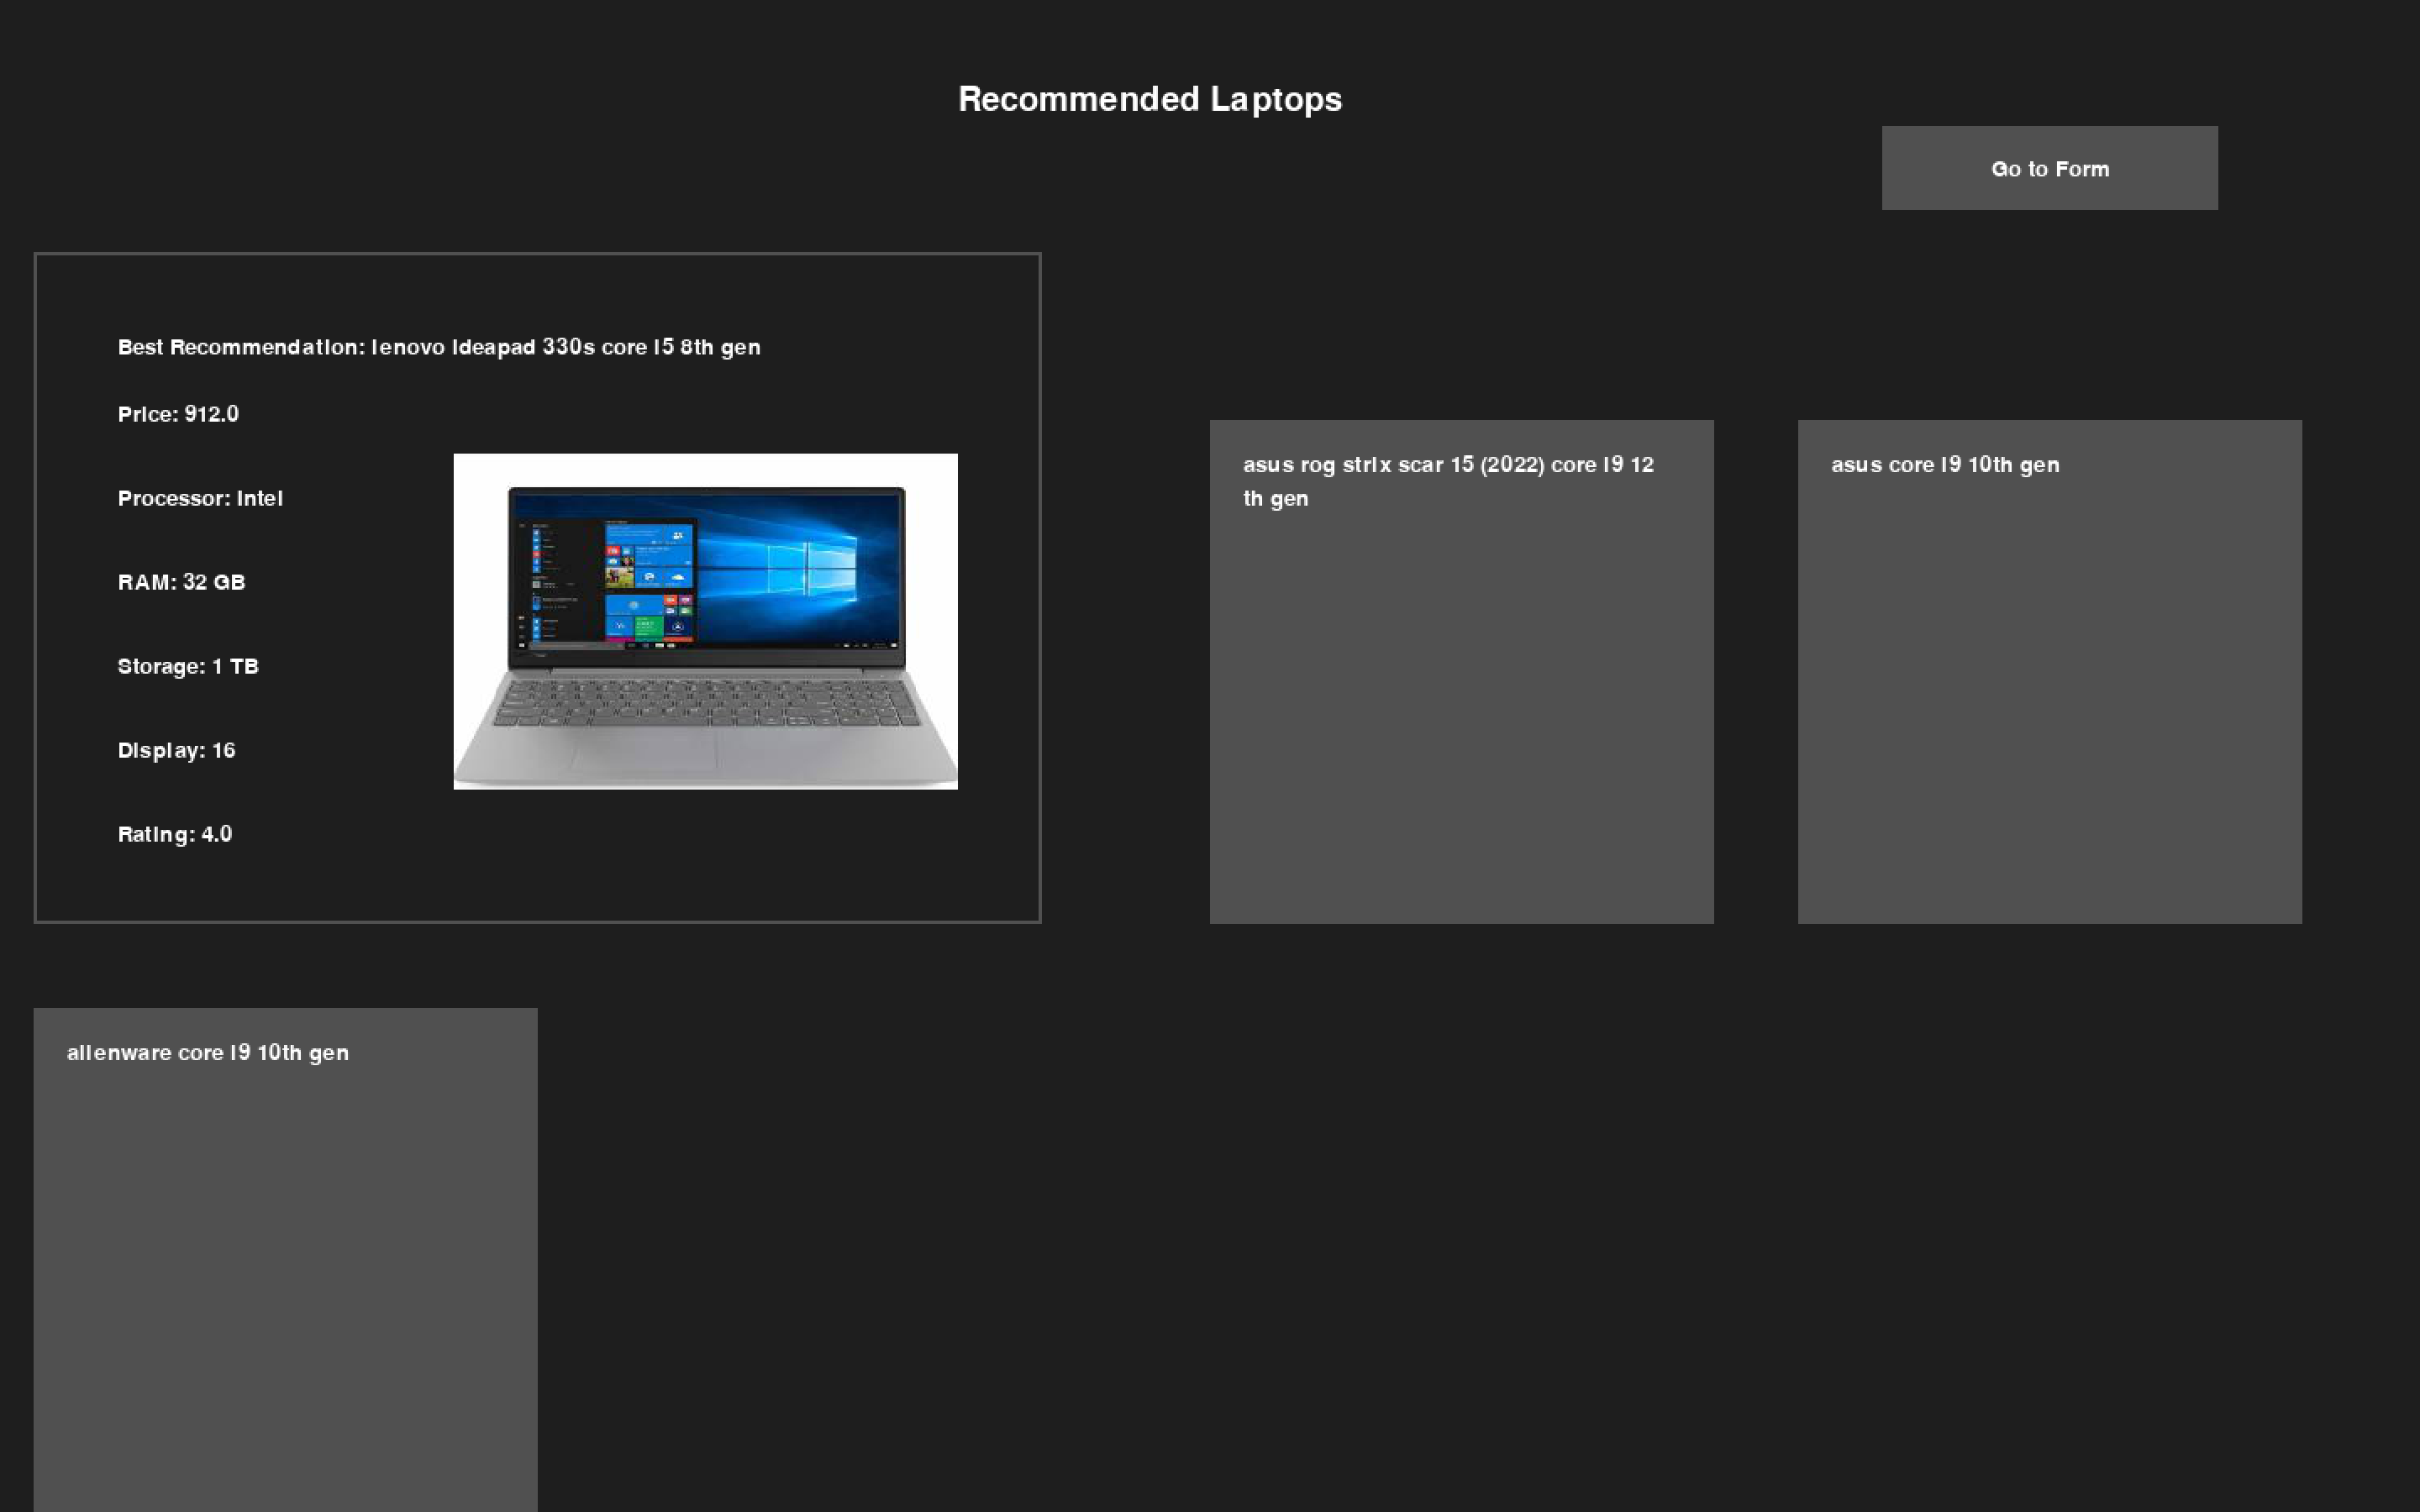
\includegraphics[scale=0.1]{proj2_output_window.png}
\\
\texttt{This is the recommended laptops screen.}
% include descriptions for screenshots

\section{Changes from project plan}
\begin{itemize}
    \item As per the TA's suggestions on our proposal, we reconsidered using a tree-ADT and changed it to utilize an unweighted graph since the decision tree approach seemed too similar to list filtering with if statements.
    \item We also considered implementing reviews within the calculation. While we could've made the graph weighted, it required too many changes to the code structure we had prepared so we opted to keep the unweighted graph. 
    \item We decided to implement a partial match system as per the TA's suggestion. Because of this, the user can choose which details to enter outside of price range and the number of laptop suggestions to show.
    \item We did not decide to opt for default values being selected on load, but instead left the text boxes empty and allowed users to enter their own input or randomize with the randomize button.
    \item We changed the categories for user input in the proposal as we found a better dataset including ratings and image links. In the proposal, we considered budget, laptop brand, CPU, RAM, SSD, HDD, and display size. In the final form, we created 'minimum price' and 'maximum price' the user would pay for a laptop to replace the 'budget' category, to get a better range for their budget. We also decided to discard the HDD category and just call the SSD 'storage' to not confuse users unfamiliar with tech jargon, since most modern laptops use SSDs anyways, although some have HDDs for additional storage. 
\end{itemize}

\section{Discussion}
\par Our project goal was to implement a graph to recommend laptops based on user inputs of price, brand, and laptop specifications. Although I think this goal was achieved through our program, there is definitely still room for improvement. The dataset had a lot of duplicates, to the point where around 30\% of the data was removed by the end of it, resulting in around 600 entries.There were also some obscure/less well known values that we removed from the dataset for better generality, but they could have also been implemented. For instance, there was a laptop with 4 TB storage, and some laptops with PCIe CPUs that we removed. The dataset also contained some dubious data, including those which weren’t actually true, for instance it claimed that one laptop in the original dataset had a 35 inch screen but when looked up online it did not, in fact, have a 35 inch screen but instead had a 13 inch screen. We used excel to remove the outlier data and duplicates, and refiltered with pandas. 
\\
\par Besides that, we tried to add pictures for all laptops to the display recommendations screen but experienced difficulties since there was an issue with images creating lag in the pygame screen since it took time to load images from the url and create image files with the requests and io modules, especially during scrolling. Thus, we chose to remove the images from the laptops except for the ‘best laptop recommendation’.
\\
\par Considering how many laptops may have similar specs and prices or ratings, it makes sense why a lot of the recommendations are not extremely accurate to what the user wanted and perhaps this could be improved with a more detailed dataset. We also could have used a weighted graph considering which spec the user deems more important, in order to create better estimations for how much prices and ratings mattered to the user, rather than just an equal weight of 1/8 of the total similarity score. 
\\ 
\par For improvement, we also could have asked for user input in terms from a drop down list and included the more obscure data, although we opted for user input through text since it was easier to implement with pygame. In addition, we could also incorporate machine learning techniques to calculate similarity scores with statistical modeling or modules like sklearn as the machine’s calculations could give more accurate scores. We can also improve on the User Interface of the form since it looks quite plain, and could be more eye-catching for the users to motivate the use of the form to get recommendations. Lastly, for the prices we separated laptops into two discrete categories ‘in budget’ and ‘not in budget’ based on whether the laptop’s price in the graph was in the range the user specified. This True or False binary is often not very accurate to the dataset values since a price specified may not even be in the graph, so a future improvement we could make is to sort based on closeness to the user’s price range above and below. 

\section{References}
CountBarracuda4447. (2024, September 27). Laptops have become essential tools in modern society (DOCX). CliffsNotes. https://www.cliffsnotes.com/study-notes/20160203 
\\\\
Yasir , Q. M. (2024, March 26). The indispensable role of laptops in today’s business world. LinkedIn. https://www.linkedin.com/pulse/indispensable-role-laptops-todays-business-world-freelance-education-2id8f 
\\\\
Raju, C. (2024, September 15). Laptop Selection Dataset. Kaggle. https://www.\\kaggle.com/datasets/rajugc/laptop-selection-dataset?resource=download
\\\\
Rodriguez, S. (2014, March 4). 1 in 10 in a survey think HTML is an STD. Los Angeles Times. https://www.latimes.com/business/technology/la-fi-tn-1-10-americans-html-std-study-finds-20140304-story.html\#axzz2v8lRihfX 
\\\\
How to load image from web URL in pygame. CodersLegacy. (2023, April 13). https://coderslegacy.com/python/load-image-from-web-url-pygame/ 

\end{document}
